\chapter{Prototype}
\label{cha:prototype}

\section{Architecture}
There are a number of possible ways to design a system to run distributed data intensive operations. Here are 
three well known approaches:
\begin{description}
\item{Conventional Approach} there is no distributed application in this case. Applications run on desktop machines
and they access data on on network stores such as NFS mounted or other distributed file systems. This is pretty much
the same thing that many users of data intensive scientific applications do today.

\item{Centralized Approach} this approach is we have a central orchestrator which users connect to it directly or
using a client to submit their operations. This is similar to the traditional client/server architecture. In 
many HPC distributed applications such as UNICORE, this would be the software which is installed on the cluster
and could have multiple other machines -as resources- under its control. The emphasis in this model is providing
a managed access to distributed computing resources.

\item{Decentralized Approach} in this approach we eliminate the orchestrator peer and the network of
application instances should collaborate in a decentralized fashion to keep track of data and control flow for each
task. This is the paradigm that we will follow in this chapter as our proposed design. 
\end{description}

\subsection{Collaborative design}
To give a better understanding of our solution one should think of it as a distributed collaborative application. 
Even though one instance of our application has same basic functionalities as multiple peers together
but it has been designed for collaboration and a single instance will only be functional if all the requested data are
available locally. Nevertheless this makes it possible to use application in standalone mode with no peers which might
come beneficial to some users with only local data.

We have picked a decentralized design, where peers will share the knowledge of running operations and existing datasets
with one another. The next stark point is that they will collaborate to accomplish one simple or complicated operation.
In terms of delegating a simple operation from a node which does not have the required data - but has received the command
to run such operation - to a node which contains the data.

\subsection{Hexagonal Architecture}
In a traditional approach toward application design we would have three tiers, i.e. client layer (GUI),
business layer (logic) and database layer. These tiers correspond to a one dimensional application architecture,
where there are only two \textit{sides} assumed to exist around application logic, client and database. However
this is not the case when we have a multi-dimensional architecture, where there are multiples input/output channels
around our business logic. In the latter case we have to use a so called hexagonal architecture. \cite{alistair}
In such an architecture applications receive signals from multiple communication means at the same time. This 
signals will trigger the appropriate internal business logic, therefore they can't be layered in one dimension.

Here is a high level view of the components of the system:

\begin{figure}[h]
  \centering
  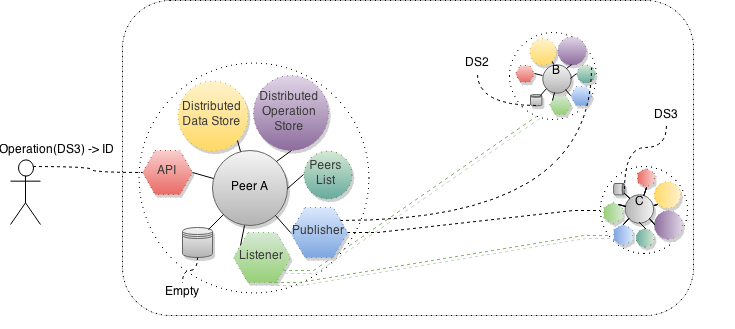
\includegraphics[width=6in]{poster/figures/sys2.png}
  \caption[High level view of a network of collaborative peers]
   {High level network view of the system}
\end{figure}

\subsection{Actors}
There are two types of actors in our problem domain.
\subparagraph{User}
A user who launches, control and monitor an operation. Typically they are employees of scientific institutes or universities.
The goal of these users is to utilize the program to launch some kind of simulation and get back the result.
\subparagraph{Instance}
Every instance can launch and observe an operation on other instances on other nodes. If we launch a single instance
network, then there would be no other instance to talk to, therefore any recursive service call will happen on the
same instance and not on any other one.
When there are more than one instance on one network, on instance has the ability to call services/operations on other
instances, basically using the same channel that one normal user does. This will make our application to act as a user
of itself. We will utilize this when we introduce recursive service calls inside our application, hence the term
\textit{collaboration}.

\subsection{Messaging}
When it comes to choosing messaging technology, the field is dominated with centralized solutions.
There are multiple solutions which bring messaging into applications, 
e.g. RabbitMQ, ActiveMQ, Celery and so on\footnote{A compelling list could be found at \url{http://queues.io/}}.
Most of them are centralized, even though they allow
distributed paradigms, their still need central servers.

Because of the nature of our application, peers might join and leave the network.
Therefore we need an transport layer which is designed having this in mind. 
We have selected ZeroMQ as our transport layer 
because it is trivial to build effective distributed messaging systems on top of that.
It is an open source project and has a very active community with hundreds of contributors. 
It is written in C programming language and has bindings for multiple programming languages including Python.
It is also multi-platform and is available on different architectures and operating systems.

\subsubsection{Supported Patterns}
ZeroMQ supports different messaging paradigms, among many others:
\begin{enumerate}
\item PUB/SUB which is publish/subscribe
\item REQ/REP which is similar to traditional client/server
\end{enumerate}
We only use publish subscribe during the course of this work.

\subsubsection{Publish/Subscribe}
Since we need to inform other peers about certain topics, we need a mechanism to inform them all together.
Any peer which is interested in other peers will \textit{subscribe} to their \textit{news channel}. 
The publish-subscribe pattern is the best way to realize this. 
ZeroMQ allows us to subscribe to any number of \textit{publisher} channels. 
Here are some important aspects of ZeroMQ publish-subscribe sockets:
\begin{itemize}
\item An application can subscribe to non-existing or non-running publishers.
\item A publisher will maintain separate queues and will keep messages for any subscribed party.
\item A publisher will simply drop the messages if there are no subscribers.
\item A publisher could have any number of subscribers.
\item A subscriber could subscribe to any number of publishers.
\end{itemize}

The above mentioned features gives let use to design distributed.
We could subscribe to peers regardless of their current state. 
They might fail and come back again but ZeroMQ will try recover and reconnect when the other peer is available.
In the other hand, the subscribers will not lose their messages if they go offline and come back online again.

\begin{figure}[h]
  \centering
  \includegraphics[width=4in]{zmq_fig4}
  \caption[Publish-subscribe pattern.]
   {Publish-subscribe pattern from ZMQ guide. \cite{zguide}}
\end{figure}

\subsubsection{Message types}
We have decided to have a number of messages which will be exchanged between peers.
Each peer will listen to all the other peers via subscribing to their news channel.
We assign a numeric id to each of these messages to identify them. 
Here is a short overview of these topics (they are called topic in ZMQ):

\subparagraph{Delegation} informs other about a request to be handled
\subparagraph{Operation update} informs others about a change in operation distributed store
\subparagraph{Pull request} ask others to download a temporary dataset from the provided endpoint

\subsubsection{Topic  Handlers}
For each of these topics there are certain topic handlers designed to maximize flexibility of application and
make it easy to introduce new topics and change topic handlers without touching or with minimum change to existing code.

\subsubsection{Topic matching}
Topic matching or message filtering is a technique as described 
in Advanced Message Queuing Protocol (AMQP) v1.0 specification\footnote{\url{https://www.amqp.org/}}.
For each peer we have one publisher channel and one subscriber channel. 
The publisher is responsible to publish any given message to all the subscribers.
If we could assign certain message types in transport layer it makes it easier
to handle them upon arrival. 
ZeroMQ provides a very basic matching algorithm for this purpose.
It prefixes a message with a number then a blank space. 

This is how a message will be published:
\begin{lstlisting}[caption={Publisher sends packed messages}]
import zmq
import msgpack
context = zmq.Context()
socket = context.socket(zmq.PUB)
# A sample local ip address
socket.bind("tcp://192.168.1.1:4000") 
message = {'id': '247506b8-09e9-40d8-968d-6f739ba802d3'}
packed = msgpack.packb(message)
# An agreed constant for operation news
topic = 10013
socket.send('%s %s' % (topic, packed))
\end{lstlisting}

\subparagraph{Messagepack} is a serializer that we use in our transport layer. 
"MessagePack is an efficient binary serialization format. 
It lets you exchange data among multiple languages like JSON.
But it's faster and smaller. 
Small integers are encoded into a single byte, 
and typical short strings require only one extra byte in addition to the strings themselves."
as described by its developers\footnote{\url{http://msgpack.org/}}.

This is how a subscriber will receive a message:
\begin{lstlisting}[language=python, caption={Subscriber receives and unpacks a message}]
import zmq
import msgpack
context = zmq.Context()
socket = context.socket(zmq.SUB)
# connecting to the publisher endpoint
socket.connect("tcp://192.168.1.1:4000")
while True:
    msg = socket.recv()
    topic, delimiter, packed = msg.partition(' ')
    topic = int(topic)
    message_dict = msgpack.unpackb(packed)
    # call appropriate handler here ..
\end{lstlisting}

\subsection{Coupling}
We have followed event driven pattern in our design.
The application components are loosely coupled and communicate using signals.

To do so we have used a Python thread-safe signaling library 
called \textit{blinker}\footnote{"Fast, simple object-to-object and broadcast signaling" -
\url{https://pypi.python.org/pypi/blinker}}.

The main cases that we use signaling is when a component wants to publish a message. 
In that case it would send a signal with corresponding topic and message. 
The publisher component will grab that signal, and will issue the real message to the peers.

In the other hand, when a new message arrives we will use dynamically registered handler objects.
Than handler will run its logic code and will notify further components by issuing corresponding signals.

Here is a basic overview of publishing process. First in sender component:

\begin{lstlisting}[language=python, caption={Publishing an internal signal with blinker}]
from blinker import signal
publish_signal = signal('publish') # signals are named
publish_signal.send(sender, {'topic': 10013})
\end{lstlisting}

The publisher component will be notified in case of a new publish message. 
This is the code that initialized the publisher upon application start:

\begin{lstlisting}[language=python, caption={Initializing the publisher upon application start}]
def _run_publisher(self):
    context = zmq.Context()
    socket = context.socket(zmq.PUB)
    socket.bind("tcp://%s:%s" % (self.ip, self.config['PUB_PORT']))
    def publish_handler(sender, topic=None, **kwargs):
	packed = msgpack.packb(kwargs)
	socket.send('%s %s' % (topic, packed))
    publish = signal('publish')
    publish.connect(publish_handler, weak=False)
\end{lstlisting}

As seen in above code snippet, the publisher assigns a function to be run when
a new signal arrives. The \textit{weak=False} is to prevent \textit{publish\_handler}
to be garbage collected when it goes out of scope with having a non-weak reference to it.

\subsection{State}
In current design we have no state machine but a number of objects have states.
The most important ones are:
\begin{itemize}
\item Operation store
\item Dataset store
\item Publisher
\end{itemize}

Operation store and dataset store are almost explained so far. 
The publisher is part of the application that has queues for each of subscribers.
In case of a failure or restart, the messages inside these queues will be discarded.

\section{Technology}
We have created a Python application using Gevent\footnote{\url{http://www.gevent.org/}},
zeromq\footnote{\url{http://zeromq.org/}} and zerorpc\footnote{\url{http://zerorpc.dotcloud.com/}} 
to be able to service multiple requests in a non-blocking way.

ZeroRPC is a remote procedure call framework which is built on top of ZeroMQ.
It is capable of exposing a given object's methods as API and made them accessible using an endpoint address.

"gevent is a coroutine-based\footnote{PEP 380 - \url{https://www.python.org/dev/peps/pep-0380/}}
Python networking library that 
uses greenlet\footnote{Lightweight in-process concurrent programming - \url{https://pypi.python.org/pypi/greenlet}} 
to provide a high-level synchronous API on top of the libev event loop."\footnote{See first footnote}


\subsection{Programming Language}
We selected Python as the main programming language to implement this project. 
There are a number of justifications to do so. Here are the main ones:

\subparagraph{Multi-Platform} Python is a multi-platform language. It runs on different operating systems
seamlessly, hence easier deployment.
\subparagraph{High Availability} Python along with its rich standard library is available by default on almost all Linux machines. This
is a great advantage for use, because we do not need to take further steps to install a runtime in highly conservative institutes.
\subparagraph{Familiarity} Python is already being used as main scripting languages in many scientific environments. This would be an advantage
for us in further steps when users want to contribute to the project or maintain it.
\subparagraph{Based on C} Python is well known to be very close to C programming languages. Even though Python is slow in arithmetic operations
it is possible to write speed critical parts in C and execute it directly within Python code. However in our current solution we do not have
arithmetic operations.
\subparagraph{Faster Development} Since Python does not need special tools to build and deploy its scripts it is much cheaper and faster
to start, build and test programs.
\subparagraph{Aspect Oriented Support} With Python it is very easy to wrap methods and apply pre-process and post-process conditions to them. We have
used this aspect of the language to create operation ids, delegate service calls, distribute messages and etc before and after service calls.

\subsection{Dependency Management} Using \textit{pip}\footnote{\url{https://pypi.python.org/pypi/pip}}
it is very trivial to manage and install multiple
dependencies of a project. It is capable of installing dependencies from remote git repositories or from 
the Python Package Index (PyPI)\footnote{\url{https://pypi.python.org/pypi}}. Moreover \textit{pip} itself is
a Python package. It gives us huge benefits with abstracting away the complexity of dependency management. It can
bundle a package with compiled dependencies, install from Python wheel\footnote{A built-package format for Python}, uninstall,
upgrade and query available PyPI packages\footnote{\url{https://pip.pypa.io/en/latest/user_guide.html}}.

\subsection{Virtual Environment}
As described in the previous section, Python is the chosen programming language for this project. Along with Python, 
comes \textit{virtualenv} package\footnote{\textit{virtualenv} is a tool to create isolated Python environments}. This is a great way of installing
project dependencies into a single directory (which serves as the virtual root file system) and avoid touching operating system managed files and
directories which normal users do not have access to them. While working inside a \textit{virtaulenv}, all the changes is written to a single directory
and all binary files, downloaded Python packages goes into that directory. Therefore this is the best way to deploy a Python project in user space.

\subsection{ZeroMQ}
The main library that powers our prototype is called ØMQ or ZeroMQ.
ZeroMQ is an asynchronous messaging library written in C with 
bindings for many languages including Python. This library helps us to easily scale and use 
different programming paradigms such as publish-subscribe, request-replay and push-pull.

\section{Key Compoenents}
We have tried to make a modular architecture with cohesive components which are loosely coupled using dynamic
method registeration. This is possible thanks to Python programming model, where functions and methods are first
class objects and we can simply pass them around. We have applied this to topic handler registeration and
internal signal handlers which we register dynamically.

\subsection{Distributed Storages}
Our aim is to distribute the information about available datasets and operations at each node. To achieve this
we let our application to launch a number of communicators and publish information about it is data.
Other nodes in our network have to subscribes on other nodes, ZeroMQ allows us to subscribe
to multiple publishers, therefore each node can subscribe to other nodes. Nodes frequently get
\textbf{news} from other nodes, for example availability of certain datasets on a node, then it
can use publish-subscribe to get extra information on that particular subject.

\subsubsection{Operation Store}
Operation store is a dictionary\footnote{In Python dictionaries 
are simple key/value objects used extensively by the language itself} 
like object that hides that distributes its content to other peers.
The interface provides getter and setter methods to explicitely add a new dataset to the store or
get an existing one.
Internally it will broadcast a specific signal along with basic information about the operation. 
It could be a newly added operation or an update to parts of the operation attributes such as a new dataset assigned
to it or about the operation entering into a new state.

\subsubsection{Dataset Store}
Currently we have only implemented a \textit{Random Dataset Store} which is similar to operation store it terms of
hiding the storage and broadcast from the rest of the application.
Meanwhile it has a few key differences.
First of all it does not have an update method. 
Beside querying the datastore, 
it only allows the application to create a new dataset and will assign a unique identifier to it.
There is currently no notion of updating a dataset.
It will publish information about the newly added dataset, 
and it will use a temporary storage to buffer the dataset and will select a random peer
and will use the networking layer to transfer the dataset to the randomly selected peer.

\subsection{Decorators}
We have used Python decorators extensively to apply pre and post processing during an operation call.

\subsection{Application}
We have capsulated the application itself as a top level class. 
A developer then would create an instance of this object and then can run it,
access the application configurations, certain public objects,
register topic handlers, ask for API endpoints, or application ports and so on.

\subsection{API}
We have made a separate API Python module\footnote{Modules in Python are simply files with .py extension which contain code}
to introduce our public API. 
We expose all the functions defined in this module as public services accessible from outside via application API port.

\begin{figure}[h]
  \centering
  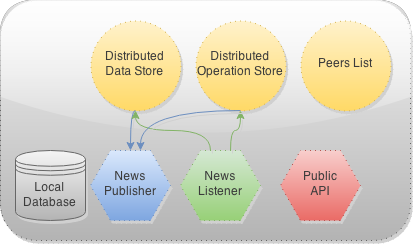
\includegraphics[width=4in]{poster/figures/sys.png}
  \caption[Another view of system compoenents]
   {Another view of system compoenents}
\end{figure}

\section{Layers}
\subsection{Network}
This layer is responsible to run the publisher channel. 
Here are the responsibilities of this layer:

\begin{itemize}
\item Exposing application public interface
\item Running publisher channel
\item Listening to internal signals to publish corresponding messages
\item Subscribing to peers
\item Getting incoming messages from subscribers 
\item Find and call appropriate handler upon arrival of new messages
\end{itemize}

\subsubsection{API}
Since this is a network program we need to use a form of Remote Procedure Call (RPC) 
to communicate between nodes. We used a library based on zeromq 
called \textit{zerorpc}. Using this library we now expose a set of APIs as services and let the nodes talk to 
each other based on this API. There are multiple solutions for exposing services which we do not discuss here.

\subsubsection{Publisher}
Publisher is a ZeroMQ socket object which is binded to one port on the running machine. 
Having endpoint of this port, other peers can subscribe to it and listen to whatever it publishes.

\subsubsection{Listener}
Listener is another type of ZeroMQ socket. 
Having connected to a publisher's endpoint address, 
we can read any incoming messages, similar to regular sockets.
But it has this feature of connecting to multiple endpoints.

\subsection{Pre-processing}
In Python we can simply wrap any function or method or even classes, inside another one.
This is realized using decorators in Python. 
Basic usage of decorator in Python is like this:

\begin{lstlisting}[caption={Pre-processing with decorators in Python}]
def delegate(func):
    @functools.wraps(func)
    def new_func(*args, **kwargs):
        # do preprocess
        # call func, if desired
        # do post process
    return new_func

# In our code:

@delegate
def a_function(an_arg, an_option=somevalue, a_flag=False):
    # some life-changing processing here...

\end{lstlisting}

As you can see, we wrapped a function only with putting \textit{@delegate} on top of it.
Now when \textit{legacy\_function} is called, the code inside the \textit{new\_func} block
will be executed first. 
There we would have access to the original function and all of its parameters. 
We can then apply any required processing. 
We can even decide to call the real function all not.
All of these without changing the caller code and makes our application very dynamic.
This way it is really trivial to write pre-processing and post-processing for any function.
We have implemented our pre and post processing using decorators.

\subsubsection{API Calls}
Since we have used zerorpc to expose our services, we have two ways of calling them.
First is using the command line tool provided along with it which has the same name.
The second is using zerorpc Python package which lets us to programmatically call
our exposed services.

Here is how we call a service from command line:

\begin{lstlisting}[language=sh, caption={Quering an API endpoint for available commands}]
\$ zerorpc tcp://127.0.0.1:9998
connecting to "tcp://127.0.0.1:9998"
list             Return a list of datasets or peers
echo             Echo
use_case_2       Invokes operation for use case 1 described \\
					in the report. Accepts 'peers', \\
					'datasets' and 'operations as option.
use_case_1       Invokes operation for use case 1 described \\
					in the report. Accepts 'peers', \\
					'datasets' and 'operations as option.
\end{lstlisting}

This is the the normal output when we provide the endpoint of one of our instances. 
We get a list of available (exposed) commands along with their documents.

Here we call a service:
\begin{lstlisting}[language=sh, caption={Running an operation on a dataset}]
\$ zerorpc tcp://127.0.0.1:9998 use_case_1 ds1
\end{lstlisting}

This would be how we get the content of operation store after calling aforementioned command:

\begin{lstlisting}[language=sh, caption={Getting list of operations}]
\$ zerorpc tcp://127.0.0.1:9998 list operations
connecting to "tcp://127.0.0.1:9998"
{'1096486d-ed28-40b6-9254-9b2006e8557d': 
  {'args': ['ds1'],
  'command': 'use_case_1',
  'duration': 5.635747909545898,
  'result_dataset_id': \\
  	'3fb9a21c-aee3-4a6a-98b0-ad0890d75686',
  'state': 'done',
  'submit_moment': 1427122073.528059}}
\end{lstlisting}

To programmatically calling a service we would use zerorpc package:

\begin{lstlisting}[caption={Connecting to an API endpoint in ZeroRPC}]
import zerorpc
c = zerorpc.Client()
c.connect("tcp://192.168.1.1:4000")
answer = c.echo('hi')
\end{lstlisting}

%\subsection{Backend}
%\subsubsection{Logic}
%\subsubsection{Stores}
%\subsubsection{Database}

\section{Initialization}
First of all each application instance establish its own zeromq publisher socket. Then it subscribes
itself to all other nodes which are listed in config file. It will also bring up the API channel.
There would be more steps such as registering handlers for various topics and preparing internal
signal handlers.
\subsection{Local Database}
For testing purposes we used a temporary HDF5 file as backend storage.
\subsection{Stores}
During initialization step we initialize our dataset store with available datasets in our HDF5 file.
\subsection{Network}
All of network initialization will be done after reading the local store.

%\section{Control Flows}
%\subsection{API Call Flow}
%\subsubsection{Possible Reactions}
%\subsection{Incoming Message Flow}
%\subsubsection{Possible Reactions}

%\section{Queries}

\section{Deployment}
The software is easily installable in a Python Virtual Environment. 
All the requirements could be installed within the virtual environment.

\section{Test Results}
To be able to assess the performance of each given solution to the mentioned scenarios we made a demo application
called \textbf{Konsensus} which its code is available on Github. \cite{konsensus}

\subsection{Integration Tests}
Writing integration tests for a distributed application is not as straightforward as writing unit-tests for a normal application. 
Our demo application acts as a server and client at the same time. Moreover we want to launch multiple 
network peers running on one or more machines. Testing scenarios on this network is not possible with
normal mocking approaches, because we need to test the behavior of our solution in a network of collaborating
peers which are not external, rather the core services of the application.

To overcome testing issues we have to launch the desired number of peers separately and then run our tests 
over them. To make this operation faster we changed the application to make it possible to launch any number
of instances on one machine and we automated this process using a number of scripts. %TODO more details

\subsubsection{Mixing Signals in Greenlets}
We use Python Greenlets instead of threads. This means that our demo application runs on only one thread. 
This causes a problem when launching multiple apps all together with one script and inside one thread, that
causes the signals for events spread among all greenlets and make trouble. To avoid this we have to run
each server in a separate processes. Running them inside threads won't help as well because the blinker Python
library is thread-safe so it moves signals between threads as well as Greenlets.

\iffalse
\subsubsection{Scenario 2 Errors}
While testing scenario 2 we observed a common error. We this scenario with three different peers as the following table:

\begin{tabular}{ l c r }
\em{Server ID} & \em{ Dataset ID} & \em{ Client} \\
S0 & --- & Yes \\
S1 & DS1 & No \\
S2 & DS2 & No \\
\end{tabular}\\

We also used \textbf{Random Dataset Storage} mechanism, simply to store resulting dataset of one operation on one of the network
peers. The problem is when two peers decide to store the result of one operation on each other a blocking condition happens. Our
approach was opening a temporary port and inform the other peer to fetch the data. 
Meanwhile this is exactly happening on the other peer, therefore both block.

\subparagraph{Solution}
To solve the blocking peers problem we used the already running main application API instead of 
opening temporary PULL/PUSH zeromq sockets. 
This change is working fine and the peers exchanging datasets with no problem.
\fi